\documentclass[twocolumn]{aastex631}

% Packages
\usepackage{microtype}  % ALWAYS!
\usepackage{amsmath}
\usepackage{amsfonts}
\usepackage{amssymb}
\usepackage{multirow}

\definecolor{pink}{RGB}{232,132,161}
\newcommand{\kc}[1]{\textcolor{pink}{\textbf{#1}} }

\newcommand{\mlg}{\ensuremath{\textrm{M}_{\rm LG}}}
\newcommand{\mmto}{\ensuremath{\textrm{M}_{\rm M31}}}
\newcommand{\mmw}{\ensuremath{\textrm{M}_{\rm MW}}}
\newcommand{\msun}{\ensuremath{\textrm{M}_{\odot}}}
\newcommand{\vtan}{\ensuremath{v_\textrm{tan}}}
\newcommand{\vrad}{\ensuremath{v_\textrm{rad}}}
\newcommand{\mud}{\ensuremath{\mu_\delta}}
\newcommand{\mua}{\ensuremath{\mu_\alpha^*}}
\newcommand{\bov}{\ensuremath{\boldsymbol{v}}}
\newcommand{\pos}[2]{\ensuremath{\boldsymbol{x}_{\rm #1 \to #2}}}
\newcommand{\vel}[2]{\ensuremath{\bov_{\rm #1 \to #2}}}
\newcommand{\mwbary}{\ensuremath{\textrm{MW}_\textrm{bary}}}
\newcommand{\mwouter}{\ensuremath{\textrm{MW}_\textrm{outer}}}
\newcommand{\mwdisk}{\ensuremath{\textrm{MW}_\textrm{disk}}}

% Style tweaks
% \renewcommand{\twocolumngrid}{\onecolumngrid}
% \setlength{\parindent}{1.1\baselineskip}
% \sloppy\sloppypar\raggedbottom\frenchspacing

%%%%%%%%%%%%%%%%%%%%%%%%%%%%%%%%%%%%%%%%%%%%%%%%%%%%%%%%%%%%%%%%%%%%%%%%%%%%%%%%
\shorttitle{Updated Local Group Mass from Timing Argument}
\shortauthors{Chamberlain, Price-Whelan et al.}

%%%%%%%%%%%%%%%%%%%%%%%%%%%%%%%%%%%%%%%%%%%%%%%%%%%%%%%%%%%%%%%%%%%%%%%%%%%%%%%%
\graphicspath{{./}{figures/}}
% Missions
\newcommand{\project}[1]{\textsl{#1}}

% Packages / projects / programming
\newcommand{\package}[1]{\textsl{#1}}
\newcommand{\acronym}[1]{{\small{#1}}}
\newcommand{\github}{\package{GitHub}}
\newcommand{\python}{\package{Python}}
\newcommand{\astropy}{\package{Astropy}}

% Stats / probability
\newcommand{\given}{\,|\,}
\newcommand{\norm}{\mathcal{N}}
\newcommand{\pdf}{\textsl{pdf}}

% Maths
\newcommand{\dd}{\mathrm{d}}
\newcommand{\transpose}[1]{{#1}^{\mathsf{T}}}
\newcommand{\inverse}[1]{{#1}^{-1}}
\newcommand{\argmin}{\operatornamewithlimits{argmin}}
\newcommand{\mean}[1]{\left< #1 \right>}

% Non-scalar variables
\renewcommand{\vec}[1]{\ensuremath{\bs{#1}}}
\newcommand{\mat}[1]{\ensuremath{\mathbf{#1}}}

% Unit shortcuts
\newcommand{\Msun}{\ensuremath{\mathrm{M}_\odot}}
\newcommand{\Mjup}{\ensuremath{\mathrm{M}_{\mathrm{J}}}}
\newcommand{\kms}{\ensuremath{\mathrm{km}~\mathrm{s}^{-1}}}
\newcommand{\pc}{\ensuremath{\mathrm{pc}}}
\newcommand{\kpc}{\ensuremath{\mathrm{kpc}}}
\newcommand{\Mpc}{\ensuremath{\mathrm{Mpc}}}
\newcommand{\kmskpc}{\ensuremath{\mathrm{km}~\mathrm{s}^{-1}~\mathrm{kpc}^{-1}}}
\newcommand{\dayd}{\ensuremath{\mathrm{d}}}
\newcommand{\yr}{\ensuremath{\mathrm{yr}}}
\newcommand{\Kel}{\ensuremath{\mathrm{K}}}

% Misc.
\newcommand{\bs}[1]{\boldsymbol{#1}}

% Astronomy
\newcommand{\DM}{{\rm DM}}
\newcommand{\feh}{\ensuremath{{[{\rm Fe}/{\rm H}]}}}
\newcommand{\df}{\acronym{DF}}

% TO DO
\newcommand{\todo}[1]{{\color{red} TODO: #1}}
\newcommand{\apw]}[1]{{\color{green} APW says: #1}}

% Projects
\newcommand{\gaia}{\textsl{Gaia}}
\newcommand{\gaiadr}{\textsl{Gaia}~\acronym{EDR3}}


% Affiliations
\newcommand{\affuofa}{University of Arizona, 933 N. Cherry Ave,
    Tucson, AZ 85721, USA}
\newcommand{\affcca}{Center for Computational Astrophysics, Flatiron Institute,
    Simons Foundation, 162 Fifth Avenue, New York, NY 10010, USA}

%% This is the end of the preamble.  Indicate the beginning of the
%% manuscript itself with \begin{document}.

\begin{document}

\title{
    A timing argument mass for the Local Group accounting for the
    Milky Way--LMC reflex motion
}

\author[0000-0001-8765-8670]{Katie~Chamberlain}
\affiliation{\affuofa}
\affiliation{\affcca}

\author[0000-0003-0872-7098]{Adrian~M.~Price-Whelan}
\affiliation{\affcca}

\author{Others!}

\begin{abstract}
    % \textbf{Context}
    The Local Group mass sets the distribution and kinematics of its constituent
    galaxies and is necessary to place it in a cosmological context.
    Though challenging to measure, one method that has been used to estimate the
    Local Group mass is the Timing Argument, which constructs a Keplerian
    orbital model that is matched to the observed kinematics of M31 with
    respect to the Milky Way.
    However, recent observations of stellar tracers in the outer MW halo have
    revealed an excess velocity dipole in the radial velocities that can be
    interpretted as a bulk motion of the Milky Way disk with respect to its
    outer halo.
    This motion of the disk has previously been unaccounted for in Timing
    Argument models.
    % \textbf{Aims}
    We aim to infer a Local Group mass that accounts for the reflex motion of
    the Milky Way disk.
    % \textbf{Methods}
    We use Bayesian techniques to fit collected datasets of 6D phase-space
    information of M31 and determine the dependence of the inferred Local Group
    mass on the magnitude of the reflex motion.
    % \textbf{Results}
    We provide an updated Local Group mass of $4.69\pm0.71 \times 10^{12}$
    \msun\ assuming a disk travel velocity of $32\rm km/s$.
    Additionally, we find that the inclusion of the reflex motion of the MW disk
    systematically lowers the inferred Local Group mass via the Timing Argument,
    and that the recovered mass depends strongly on the assumed travel velocity
    of the disk.
    Further measurements of the reflex motion of the disk will likely yield a
    larger observed travel velocity, and therefore a lower Local Group mass.
    In addition, improvements to proper motion measurements from future Gaia
    data releases may improve the constraint on the Local Group mass by a factor
    of $\sim2$.
    % \textbf{Conclusions}
    The Timing Argument remains one of the only ways to measure the Local Group
    mass independently of the masses of the individual component galaxies, but
    it is clear that the effect of the LMC must be accounted for when using
    these techniques.

\end{abstract}

\section{Introduction}
\label{sec:intro}

\begin{itemize}
    \item The mass of the local group is a fundamental quantity in many local
    cosmological and Milky Way applications
    \item cosmological impact
        \begin{itemize}
            \item bias and calibration of the timing argument
            \item what a lower/higher group mass means (we're gonna be more consistent w other group mass measurements, I think?)
        \end{itemize}
    \item ways to measure local group mass: \begin{itemize}
            \item (summarize other methods, non-TA)
            \item introduction of timing argument
          \end{itemize}
    % \item what's wrong with previous use of TA?
    %     \begin{itemize}
    %         \item the LMC is massive and pulling on the MW disk
    %         \item previous use of timing argument did not account for travel velocity of the disk
    %         \item we include the travel velocity of the disk
    %     \end{itemize}
\end{itemize}


%%%%%%%%%%%%%%%%%%%%%%%%%%%%%%%%%%%%
\section{The Timing Argument}
\label{sec:timingarg}
%%%%%%%%%%%%%%%%%%%%%%%%%%%%%%%%%%%%

Following past work \citep[e.g.,][]{Lynden-Bell:1981, vdm2012, Penarrubia2016},
we assume that the orbital trajectories of the M31 and MW --- the Local Group
system --- over cosmic history are well-described by Keplerian orbits.
By assuming that the M31 and MW are gravitationally bound and were last at
closest approach in the early universe (i.e. the two galaxies have not yet
strongly interacted), we can then use the present-day kinematics of M31 to
estimate the total mass of the Local Group (i.e. using the ``Timing Argument'').

% \textbf{The dynamics of the M31-MW system can be approximated by simple Keplerian orbits.}
We largely follow the methodology and notation defined in
\citet{Penarrubia2016}, but the Timing Argument has been used in many other
studies \citep[e.g.,][]{stuff}.
% TODO: we have to put a list of TA references here so people don't get
% grumpy... but they will still be grumpy!
Briefly recapping the Timing Argument method, we assume that the dynamics of the
MW and M31 is dominated by the local gravitational potential of the Local Group
(LG) and therefore the Hubble flow can be neglected for computing the relative
orbits of the galaxies \citep[see, e.g.,][]{someone}.
% TODO: figure out most relevant citation for this!
Since we observe something close to the relative position and motion between M31
and the MW, we reduce the dynamics of the galaxies in the LG system to a single
Keplerian orbit that specifies the relative orbit between the galaxies and is
completely determined by four model parameters: the total mass of the Local
Group \mlg, the semi-major axis $a$, the eccentricity $e$, and the present value
of the eccentric anomaly $\eta$.

In terms of these four model parameters, the closed-form equations for relevant
two-body quantities like the separation between the masses $r$, the elapsed time
since last pericenter $t$, and the radial and tangential velocity components
\vrad\ and \vtan\ are given by:
\begin{align}
  r &= a \, (1-e\,\cos\eta) \label{eq:r} \\
  t &= \left( \frac{a^3}{GM} \right)^{1/2}(\eta-e\,\sin\eta) \label{eq:t} \\
  \vrad &= \left( \frac{GM}{a} \right)^{1/2} \frac{e\,\sin\eta}{1-e\,\cos\eta} \label{eq:vrad} \\
  \vtan &= \left( \frac{GM}{a} \right)^{1/2} \frac{\sqrt{1-e^2}}{1-e\,\cos\eta} \label{eq:vtan} \quad .
\end{align}
In our model, the separation $r$ is the distance between the centers of mass of
M31 and the MW, the time since last pericenter $t$ is the age of the Universe,
and (\vrad, \vtan) expresses the radial and tangential velocity components of
M31 relative to the MW center.

In a simpler universe where the MW and M31 are point masses and there are no
other massive bodies in the LG system, we could transform the observed
heliocentric sky position, distance, and velocity of M31 to a MW Galactocentric
reference frame and combine these with an estimate of the Hubble time to obtain
the four ``observables'' $(r, t, \vrad, \vtan)$ and then infer the four model
parameters $(\mlg, a, e, \eta)$ using Equations~\ref{eq:r}--\ref{eq:vtan}.
% \textbf{To compare our model predictions of the M31-MW system to the observed kinematics, we must translate these quantities into observables to constrain our model with observational data.}
To describe this ``classical'' Timing Argument approach in more detail and set
the stage for extending it, we adopt the notation of \citet{Penarrubia2016} in
which $\vel{A}{B}$ represents the velocity vector of A as measured in
the reference frame of B and $\pos{A}{B}$ represents the position vector of A as
measured from B.
With this notation, $\vel{A}{B} = -\vel{B}{A}$ and $\vel{A}{C} = \vel{A}{B} +
\vel{B}{C}$.
Thus, the position and velocity of M31 with respect to the center of mass of the
MW can be represented by $\pos{M31}{\mwbary}$ and $\vel{M31}{\mwbary}$
respectively, and the position and velocity of M31 as measured in a heliocentric
reference frame are given by
\begin{align}
  \pos{M31}{\odot} &= \pos{M31}{\mwbary} + \pos{\mwbary}{\odot} \label{eq:xoffset1}\\
  \vel{M31}{\odot} &= \vel{M31}{\mwbary} + \vel{\mwbary}{\odot} \label{eq:voffset1}\quad .
\end{align}
Here $\left|\pos{M31}{\mwbary}\right| = r$, $\vel{M31}{\mwbary}$ is determined
completely by the Keplerian model parameters (through \vrad\ and \vtan), and the
position and velocity of the center of mass of the MW as measured from the sun
are $\pos{\mwbary}{\odot}$ and $\vel{\mwbary}{\odot}$, respectively, and are
given by the adopted solar position and velocity in the Galaxy (the values we
adopt are given in Section~\ref{sec:datasets} below).

As noted above and in \citet{Penarrubia2016}, the dynamics of the MW--M31 system
is now thought to be more complex because of the infall of the LMC into the MW's
dark matter halo:
It is thought that the recent pericentric passage of the LMC has, to first
order, imparted a velocity boost on the disk and central regions of the MW,
shifting its position and velocity with respect to the mean position and
velocity of tracers in the outer MW \citep{Nico, Erkal, Petersen}.
This implies that we must account for additional terms in
Equations~\ref{eq:xoffset1} and \ref{eq:voffset1} to account for the reflex
motion of the MW disk with respect to the outer halo.
Thus, the observed position and velocity vector of M31 from the solar reference
frame is instead given by
\begin{align}
  \pos{M31}{\odot} &= \pos{M31}{\mwouter} + \pos{\mwouter}{\mwdisk}+\pos{\mwdisk}{\odot} \\
  \vel{M31}{\odot} &= \vel{M31}{\mwouter} + \vel{\mwouter}{\mwdisk}+\vel{\mwdisk}{\odot}
\end{align}
where ``\mwouter'' refers to a reference frame centered at and moving with the
center of mass of the outer MW halo and ``\mwdisk'' refers to a reference frame
centered at and moving with the center of the MW disk.
We assume that the outer MW halo frame is equivalent to the MW barycentric frame
in the simpler case where there is no LMC, or in other words we assume that the
outer MW halo has not yet had time to respond to the infall of the LMC.
We also assume that the sun, Galactic disk, and inner MW moved as a solid body
so that $\vel{\mwdisk}{\odot}$ and $\vel{\mwdisk}{\odot}$ are equivalent to the
solar position and velocity with respect to the Galactic center (as in
Equations~\ref{eq:xoffset1}--\ref{eq:voffset1}).
Figure~\ref{fig:schematic} shows a schematic of these different vectors --- all
drawn in a frame that is comoving with the \mwouter\ frame --- and a rough
illustration of the geometry we assume.

In what follows, we will assume that we have access to a direct measurement of
$\vel{\mwouter}{\mwdisk}$; This is different from \citet{Penarrubia2016} who
instead parametrize this term as a function of an additional parameter that sets
the mass ratio of the LMC and the MW.
We also assume that $\pos{\mwouter}{\mwdisk} \approx 0$ motivated by the fact
that this displacement is likely much smaller than the distance between the MW
and M31 $\pos{\mwouter}{\mwdisk} \ll r$ \citep[as expected from simulations,e.g.,][]{Garavito-Camargo2021b}.

% APW: I'm not sure we need to go into detail about the coordinate system here
% info about coordinate system setup
% \textbf{We choose a coordinate system centered on the disk of the MW, where positive x is along the line of sight between the MW disk and the center of M31's disk, and positive y is in the direction of the tangential motion of M31.} Thus, the velocity vector of M31 in this Keplerian coordinate system is $(v_x, v_y, v_z) =(v_{rad},v_{tan},0)$, and $v_{rad}<0$ means M31 is moving towards the MW disk.

%%% Schematic %%%
\begin{figure*}[htb]
  \centering
  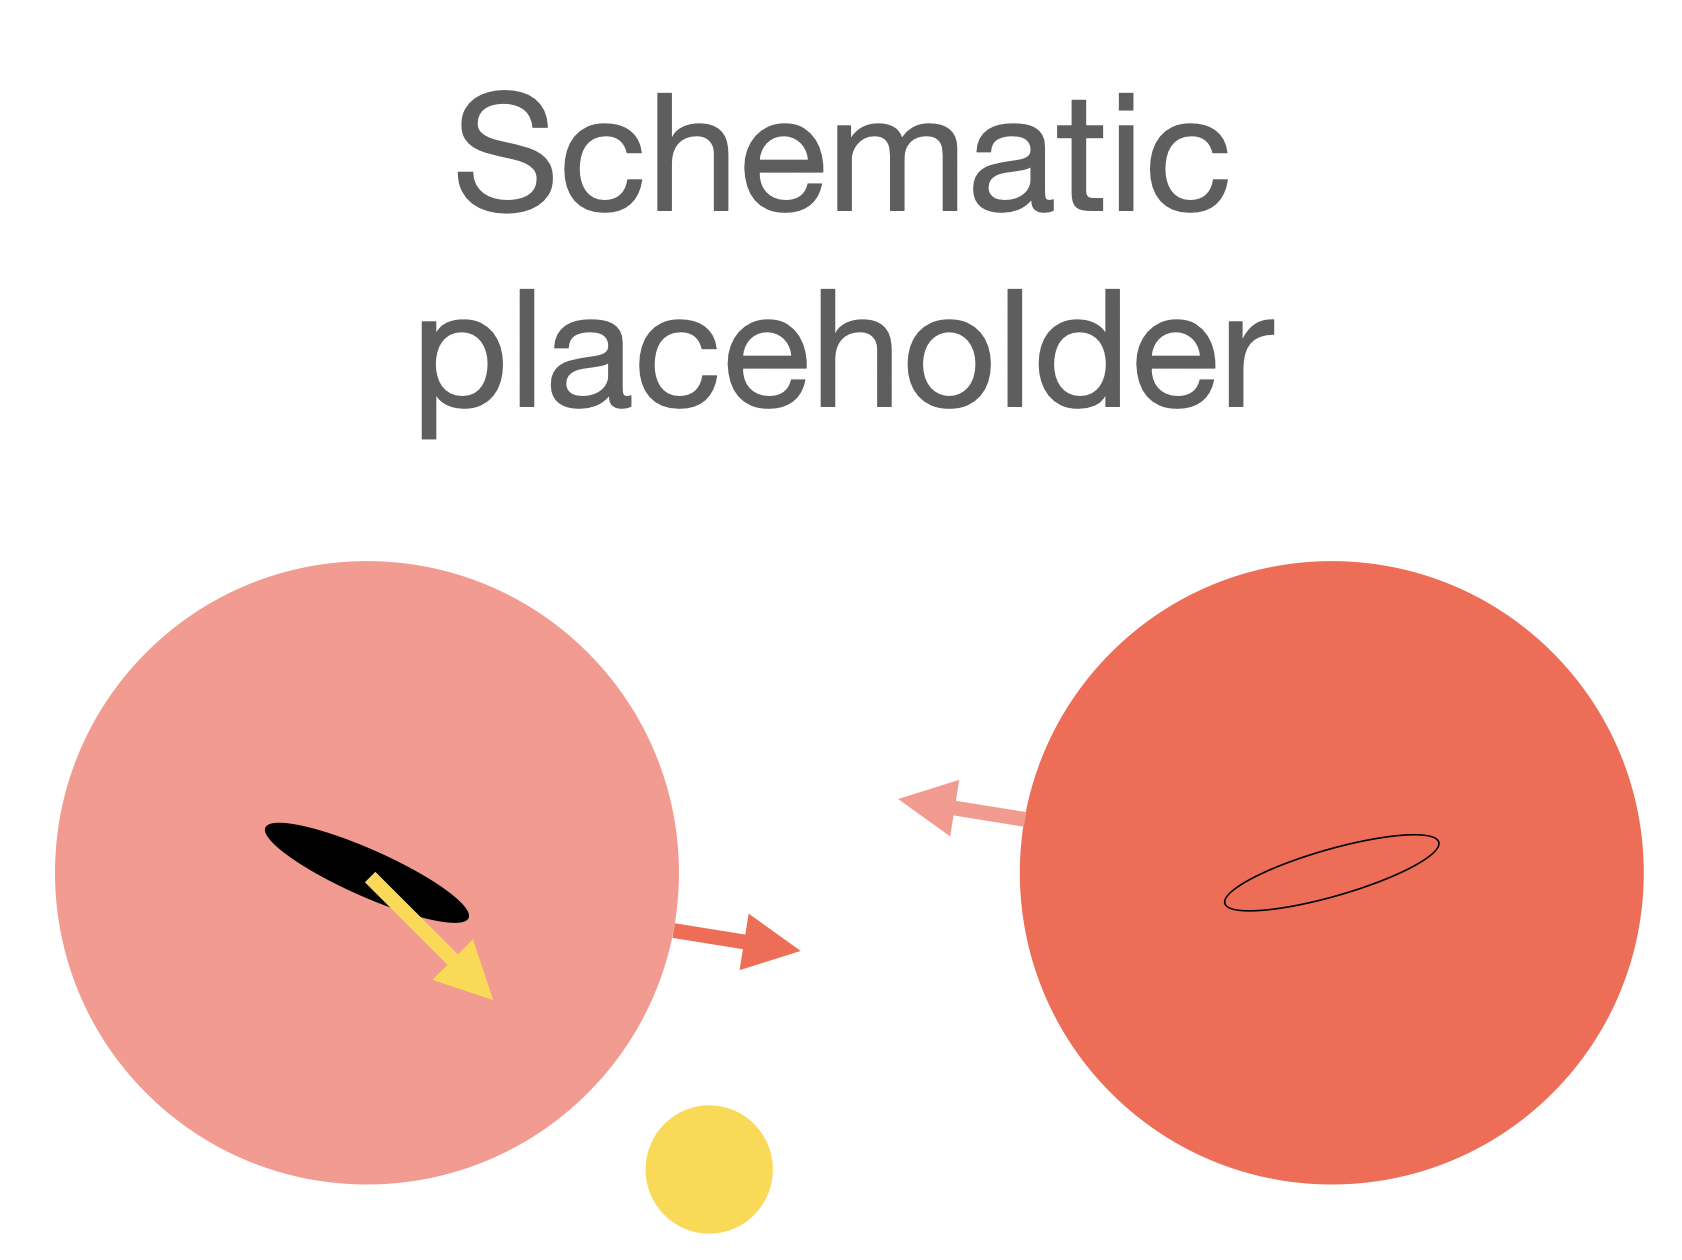
\includegraphics[width=0.8\columnwidth]{schematic_placeholder.png}
  \caption{
    Placeholder for whatever schematic we're going to end up creating
  }
  \label{fig:schematic}
\end{figure*}


%%%%%%%%%%%%%%%%%%%%%%%%%%%%%%%%%%%
\section{Datasets}
\label{sec:datasets}
%%%%%%%%%%%%%%%%%%%%%%%%%%%%%%%%%%%

Key input into Timing Argument inferences of the Local Group mass are the
present position and velocity of M31 and the age of the universe (used in in
Equation~\ref{eq:t}).
Here we consider two compilations of data that provide this information to have
as comparisons.
The two datasets used in our analysis are summarized in Table~\ref{table:data}.
Briefly, ``Dataset 1'' comes from the measured proper motion of M31 and a
collection of other data used to constrain the mass of the Local Group via the
Timing Argument in~\citet{vdm2012}.
``Dataset 2'' is a compilation of more recent measurements, including a more
precise Cepheid-based distance measure to M31 \citep{Li2021} and updated proper
motions of M31 measured using data from \textit{Gaia} eDR3 \citep{Salomon2021}.
The \textit{Gaia}-based M31 proper motion measurement is slightly higher,
leading to an increased implied transverse velocity that will likely lead to a
higher inferred Local Group mass compared to the more radial orbit implied by
Dataset 1.

\begin{table*}
  \centering
  \begin{tabular}{lc|c}
    \hline\hline
                    & Dataset 1                     & Dataset 2 \\\hline
  $D$               &  770 $\pm$ 40 \rm kpc\cite{}     &   761$\pm$11 \rm kpc~\citep{Li2021}        \\
  $v_{\rm rad}$     &     -301$\pm$1 km/s       &   -301$\pm$1 km/s        \\
  ($\mu_\alpha^*$,  $\mu_\delta$)    & (44.6$\pm$12.66, -32.1$\pm$12.21) $\mu$as/yr \citep{} & (48.98 $\pm$10.47, -36.85$\pm$8.03) $\mu$as/yr \citep{Salomon2021}\\
  (U$_{\rm pec}$, V$_{\rm pec}$+V$_0$, W$_{\rm pec}$) & (11.1, 251.54, 7.25) km/s& (12.9, 245.6, 7.78) km/s \citep{Drimmel2018}\\
  $t_{\rm peri}$ & 13.75$\pm$0.11 Gyr ~\citep{Jarosik2011} & 13.801$\pm$0.024 Gyr~\citep{??}\\
  %              &           &           \\
  %              &           &           \\
  \hline\hline

  \end{tabular}
  \caption{\label{table:data}Observational datasets used for comparison throughout analysis. Each value is measured for M31 with respect to the sun. $D$ is the distance, $v_{\rm rad}$ is the radial velocity, $(\mu^*_{\alpha}, \mu_{\delta})$ are proper motions in RA cosdec and Dec, and (U$_{\rm pec}$, V$_{\rm pec}$+V$_0$, W$_{\rm pec}$) the solar motion with respect to the galactic center. $t_{\rm peri}$ is the time elapsed since the last pericenter of the M31 Keplerian orbit, which in this case is the age of the Universe. }
\end{table*}


%%%%%%%%%%%%%%%%%%%%%%%%%%%%%%%%%%%%
\section{Bayesian Inference}
\label{sec:bayes}
%%%%%%%%%%%%%%%%%%%%%%%%%%%%%%%%%%%%

We construct a likelihood function for the observed, heliocentric position and
velocity of M31 and the time since last pericenter given the four parameters of
the Timing Argument model $(\mlg, a, e, \eta)$, assign prior probability
distribution functions (pdfs) for the parameters, and use these to compute the
posterior pdf over the parameters given the data.
In detail, we first use the four Timing Argument parameters to compute the
present day separation between the MW and M31, and the relative radial and
tangential velocities as defined in Equations~\ref{eq:r}--\ref{eq:vtan}.
These velocity components represent the relative velocity M31 would have as
observed from the barycenter of the MW--LMC subsystem; We then use the measured
``travel velocity'' of the MW disk $\vel{\mwouter}{\mwdisk}$ to compute the
relative velocity of M31 that would be observed from a frame moving with the
center of the Milky Way disk (i.e. a Galactocentric frame).
We finally then transform from this Galactocentric frame to a heliocentric
reference frame moving with the solar system barycenter (i.e. ICRS coordinates).
At this final stage, we must introduce an additional nuisance parameter $\alpha$
which represents the orientation of the MW--M31 orbital plane as it intersects
the tangent plane located at the sky position of M31 on the celestial sphere.
This is necessary because the Kepler equations only provide the magnitude of the
tangential velocity (i.e. Equation~\ref{eq:vtan}), but in order to compute
proper motion components we must also know the exact orientation of the M31
velocity vector.

We specify this model using the \texttt{Python} probabilistic programming
package \texttt{pymc3}~\citep{Salvatier2016} and our adopted prior pdfs are
summarized in Table~\ref{table:priors}.
We use the No-U-Turn Sampler (NUTS) \citep{gelman?} implemented in
\texttt{pymc3} to generate samples from this posterior pdf, given data from each
of the datasets defined in Table~\ref{table:data}.
We sample over the parameter Local Group mass $\mlg$, (true) present-day MW--M31
separation $r$, log eccentricity $\ln\left(1 - e\right)$, eccentric anomaly
$\eta$, and the orbital plane orientation nuisance parameter $\alpha$.
However, we set the priors as follows:
\begin{itemize}
  \item Mass of the Local Group $\mlg$: we use a broad, truncated normal
  distribution centered on a past measured value of the local group mass.
  \item Present MW--M31 separation $r$: we again use a broad, truncated normal
  distribution centered on past measurements of the distance to M31.
  % TODO: oops - we should center it on ~770 ot 750, not 700 kpc like we chose!
  \item Eccentricity $e$: we assume a uniform prior on eccentricity but sample
  in the transformed parameter $\ln(1-e)$ to improve the acceptance fraction
  when generating posterior samples.
  \item Eccentric anomaly $\eta$: we assume a uniform prior.
  \item Orbital plane orientation $\alpha$: we assume a uniform prior.
\end{itemize}

For each dataset, we run the sampler with 4 chains for 4000 tuning steps and
8000 draws.

% \begin{equation}
%   \mathcal{L}(| \boldsymbol{S})
% \end{equation}
% where $\boldsymbol{S} = ($\mlg$, a, e, \eta)$

% TODO: Letters have a 1 table max limit, so we might have to move the prior
% details into the list above. But we could always submit as a short regular
% paper instead of a letter...
\begin{table}
  \centering
  \begin{tabular}{lc}
  \hline\hline
  Prior  & Description \\\hline
  \mlg: $\mathcal{N}(4.5,3)\times10^{12}\msun$ & Mass of the Local Group\\
  %
  $r$: $\mathcal{N}(700,100)$kpc & Distance from M31 to $\mwdisk$\\
  %
  $\ln(1-e)$: $\mathcal{U}$(-10,0) & Eccentricity (close to 1) \\
  %
  $\eta$: angle(0,2$\pi$)& Eccentric anomaly\\
  \multirow{2}{*}{$\alpha$: angle(0,2$\pi$)} & Angle between M31 orbital\\
  & pole and Galactocentric\\
  \hline\hline
  \end{tabular}
  \caption{\label{table:priors}Priors \kc{note: on \mlg and $r$, we also set bounds? how should I show those here? or should they go in the text?}}
\end{table}


%%%%%%%%%%%%%%%%%%%%%%%%%%%%%%%%%%%
\section{Results: Local group mass estimates}
%%%%%%%%%%%%%%%%%%%%%%%%%%%%%%%%%%%
\label{sec:results}
\kc{Include the velocity vector of M31 from the halo frame?}

% We use recent measurements of the present-day kinematics of M31 as observed from the solar system, updated measurements of the solar position and motion with respect to the Milky Way center, and a recent measurement of the velocity of the Milky Way disk with respect to the outer stellar halo to measure the mass of the Local Group using observed kinematics of M31.

We use a Bayesian model to place constraints on the mass of the Local Group and the distance between M31 and the Sun using the Timing Argument. Our model of the Local Group includes the reflex motion of the Milky Way disk and results in new constrains on the mass of the Local Group to 4.69$\pm0.71 \times 10^{12}\msun$.

% this will maybe go in discussion?
Previous studies that have used the Timing Argument to constrain the mass of the Local Group have found a range of masses. ~\cite{vdm2012} used the timing argument with Dataset 1 and derived a mass of $4.27\pm 0.53\times 10^{12}\msun$) \kc{note: our value of \mlg is $\sim$.3 times higher than found in vdm2012 with the same set of data with no travel velocity. probably just in implementation of mcmc or something?}.
~\cite{Penarrubia2016} finds a Local Group mass of ($\sim2.64\pm0.4\times 10^{12}\msun$) which is significantly lower than our expectations, although this constraint combines the observed kinematics of 35 Local Volume galaxies and the dynamics of the M31-MW system. Fitting for the distances and velocities of the 35 LV galaxies drastically lowers the inferred Local Group mass compared to the Timing Argument.


We found that, for both considered datasets, our model prefers lower Local Group masses and a lower eccentricity orbit compared to models that do not include MW disk reflex motion. Fig.~\ref{fig:contour} shows the 95\% contours from the sampled posterior PDFs of the distance to M31, the eccentricity of the orbit of M31 with a fixed MW, and the inferred Local Group mass. Arrows in the bottom left panel of the corner plot indicate the shift to lower masses and eccentricities when introducing the reflex motion of the MW.

The direction of the motion of the disk is directly tied to the behavior of the inferred mass of the Local Group. In this case, the orbit of the LMC and location of the LMC at pericenter are in the same region of the sky as M31 such that the radial component of motion is in the direction of M31. Thus, the observed radial velocity of M31 will be higher than for an unperturbed MW halo. Since $-v_{rad}\propto M^{1/2}$ for an infalling system, a smaller (but still negative) radial velocity will yield a lower Local Group mass.

The eccentricity decreases significantly for Dataset 2 compared to Dataset 1, due to the larger measured proper motions of Dataset 2.  Additionally, a smaller radial velocity corresponds to a lower eccentricity for a fixed mass and distance, which can be seen in the bottom right panel of~\ref{fig:contour}.

Constraints on the distance to M31 remain roughly unchanged for both datasets, primarily because our model does not introduce a physical displacement of the MW disk, since we assume the motion of the disk over the past XX Myr since the LMC achieved pericenter is negligible compared to the separation between M31 and the MW. Thus, the inclusion of the reflex motion of the disk in our model does not affect constraints on the distance to M31.


% bit about the stellar halo tracers and different distances etc
\cite{Garavito-Camargo2021b} showed that stellar halo tracers at different distances from the MW disk center may result in different measured travel velocities, and it's likely that the current measurements on $v_{travel}$ of 32km/s are just a lower bound on the actual reflex motion of the disk. In Fig.~\ref{fig:mvsv}, we show that for increasing travel velocity magnitudes, the mass of the Local Group from the Timing Argument steadily decreases. Thus, future measurements of the travel velocity of the disk will likely result in a lower inferred Local Group mass. Vertical lines show the travel velocities that are expected for three tracer distances in simulations from~\cite{Garavito-Camargo2021b}. \kc{why does the mass level off after 80kpc / 70km/s? }

% bit about PM improvement
Of all our observational data, the proper motions have the largest relative errorbars. In order to determine how improved constraints on the proper motions from future Gaia data releases would impact Timing Argument constraints on the Local Group mass, we redid our analysis as a function of the fractional improvement in proper motion errors.
We find that as proper motion measurements improve by a factor of $\sim2$, the constraints on the Local Group mass from the timing argument will improve by a factor of more than 1.5. These results are compiled in Fig.~\ref{fig:mvspm}.


\begin{figure*}[htb]
  \centering
  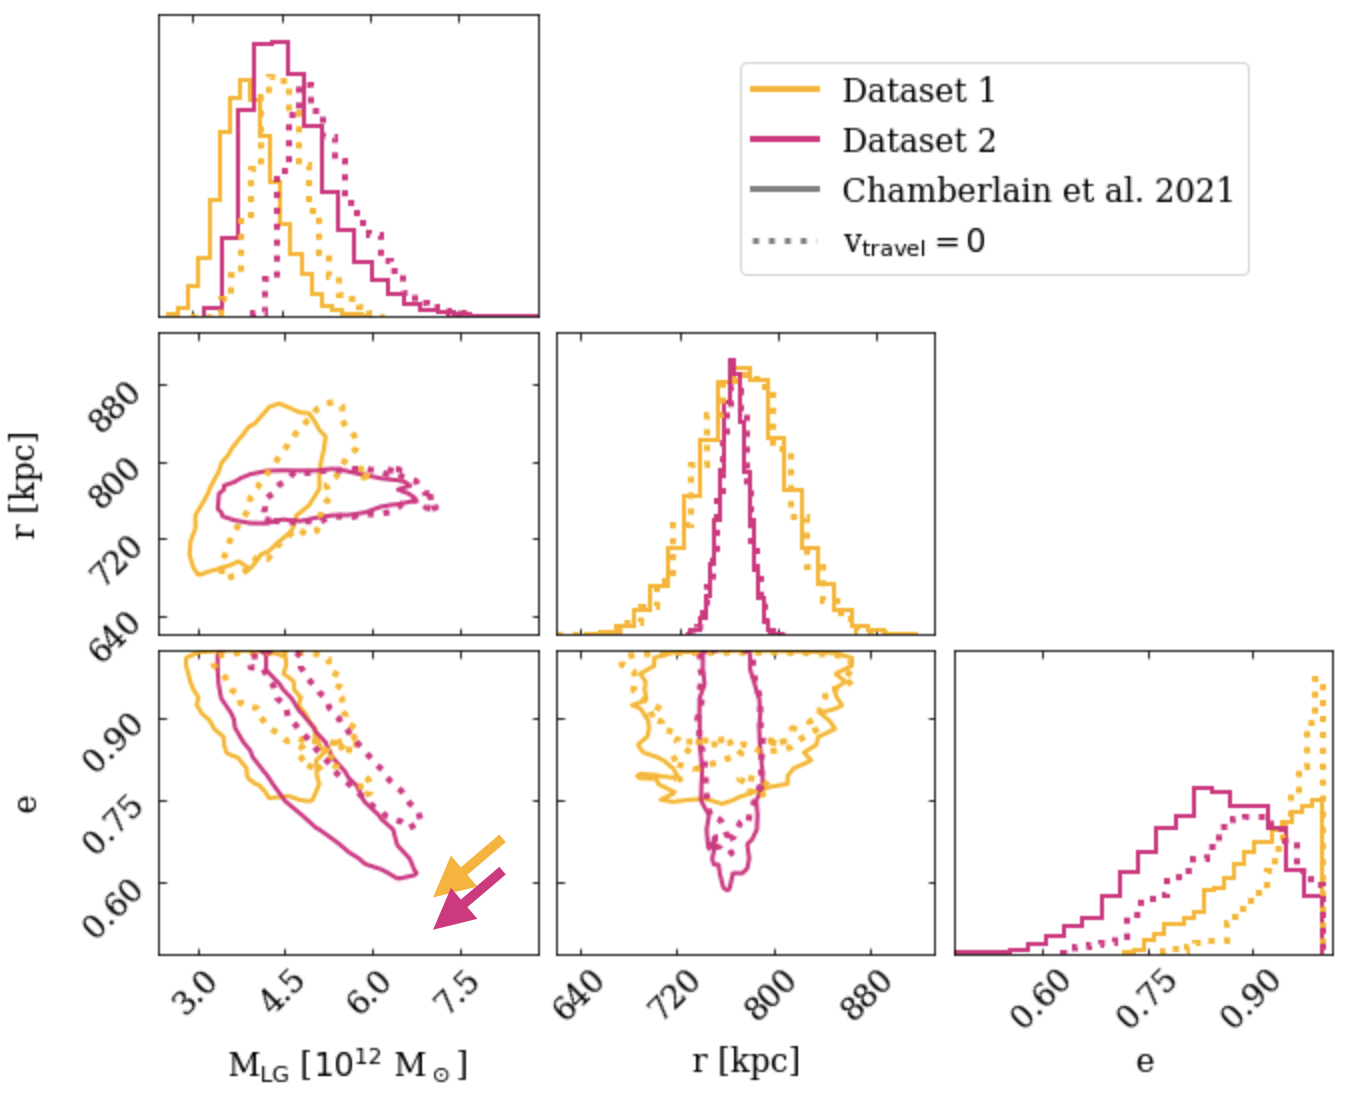
\includegraphics[width=0.8\textwidth]{analyze-runs-contour-arrows.png}
  \caption{\label{fig:contour} 95\% contours of sampled posterior distributions for two observational datasets (pink and yellow) of a subset of our model parameters: the total mass of the Local Group (\mlg), the distance between the Sun and M31 ($r$), and the eccentricity of the orbit of M31 about a fixed MW ($e$). A stationary MW disk is shown in the dotted contours, while our model, which includes the reflex motion of the MW disk, is shown in solid lines.
  The distributions for the separations are unchanged between models, as our model does not implement a spatial shift to the location of the MW disk. A comparison between the two models shows that \textbf{the inclusion of the reflex motion of the MW disk systematically lowers the inferred mass of the Local Group} regardless of observational dataset. See text for discussion on the effects on eccentricity.
  \kc{should I change this plot to have color represent our model and grey be no travel velocity?, also should I only include 2 sets of contours (68 and 95) instead of just 95? also not rn this is a bad quality screenshot but didn't know how to put arrows on the figure w matplotlib because it's using subplots as part of \texttt{corner}}  }
\end{figure*}

\begin{figure}[htb]
    \centering
    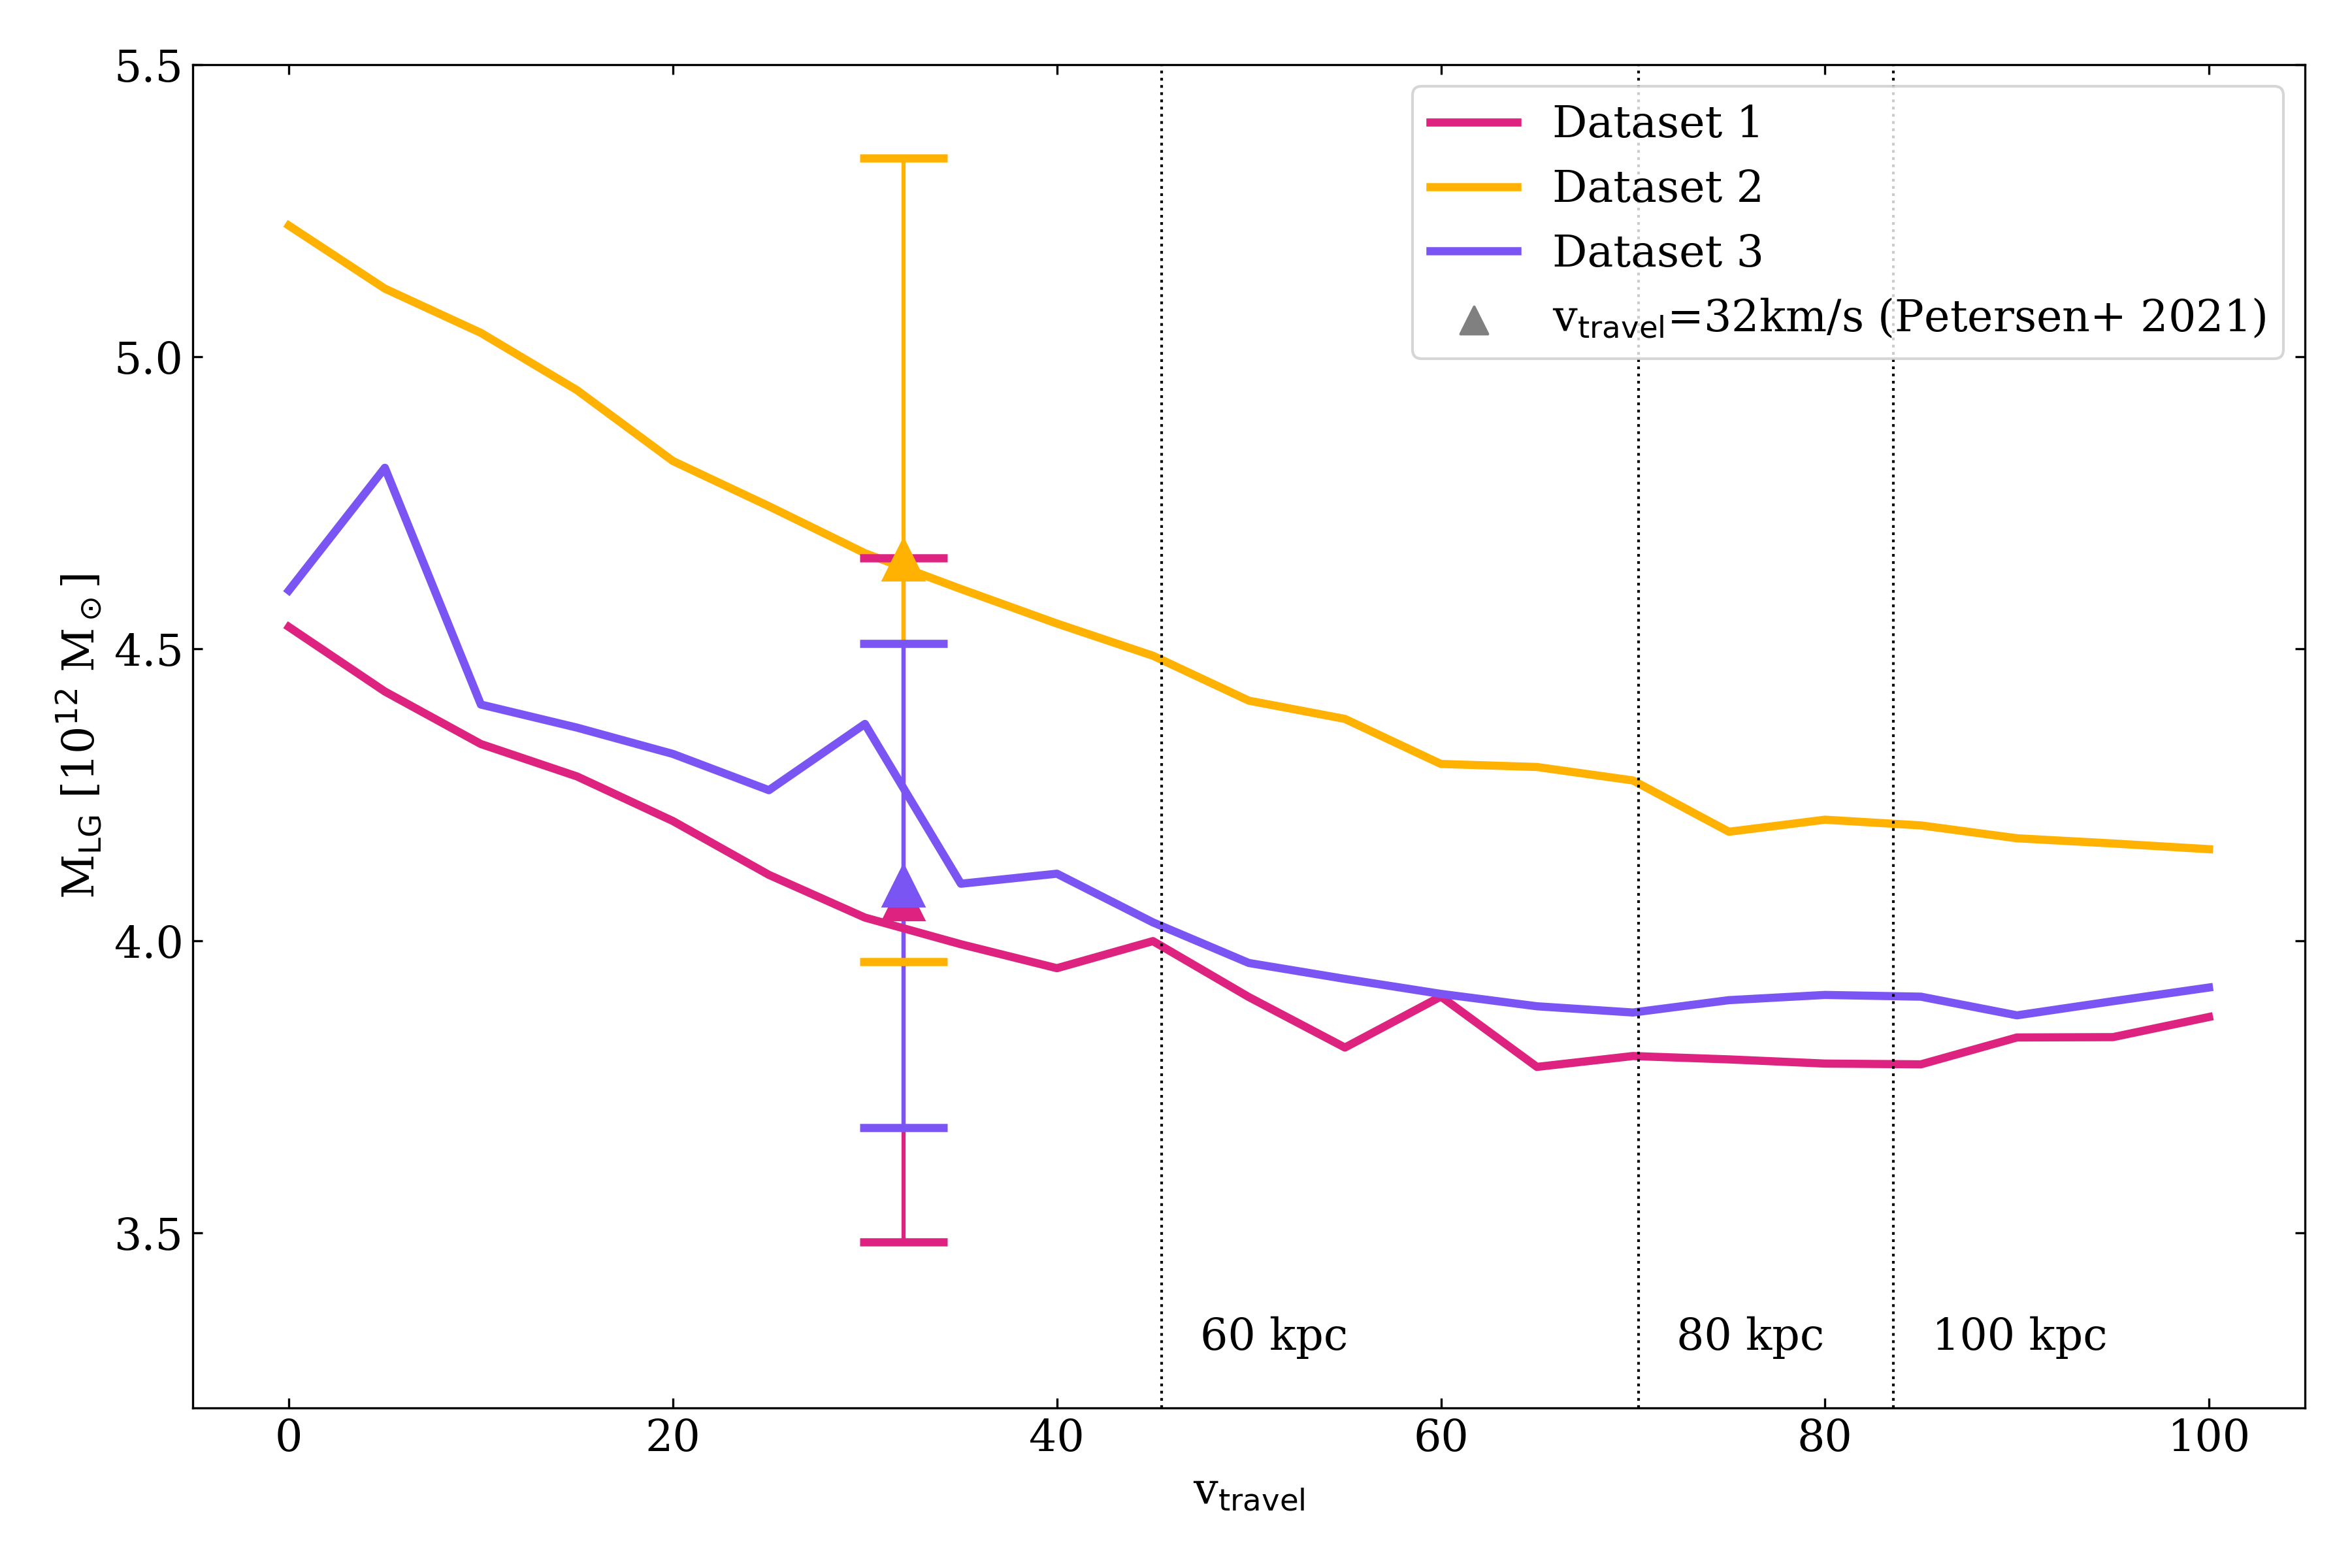
\includegraphics[width=\columnwidth]{analyze-runs-MvV.png}
    \caption{\label{fig:mvsv} Mean inferred Local Group mass as a function of travel velocity magnitude of the MW disk. Dataset 1 (yellow) yields masses that are systematically lower than Dataset 2 (pink), though they display the same general trends with increasing travel velocity. The vertical lines represent simulated travel velocities for stellar tracers at different distances in~\cite{Garavito-Camargo2021b}.
    The mean Local Group mass corresponding to the observed travel velocity from~\cite{Petersen2021} of 32km/s by the triangle points, including the 1-$\sigma$ spread on the mass at that travel velocity. \textbf{As the travel velocity of the Milky Way disk increases, the inferred Local Group mass decreases} before leveling off around 80km/s.
    }
  \end{figure}

\begin{figure}[htb]
    \centering
    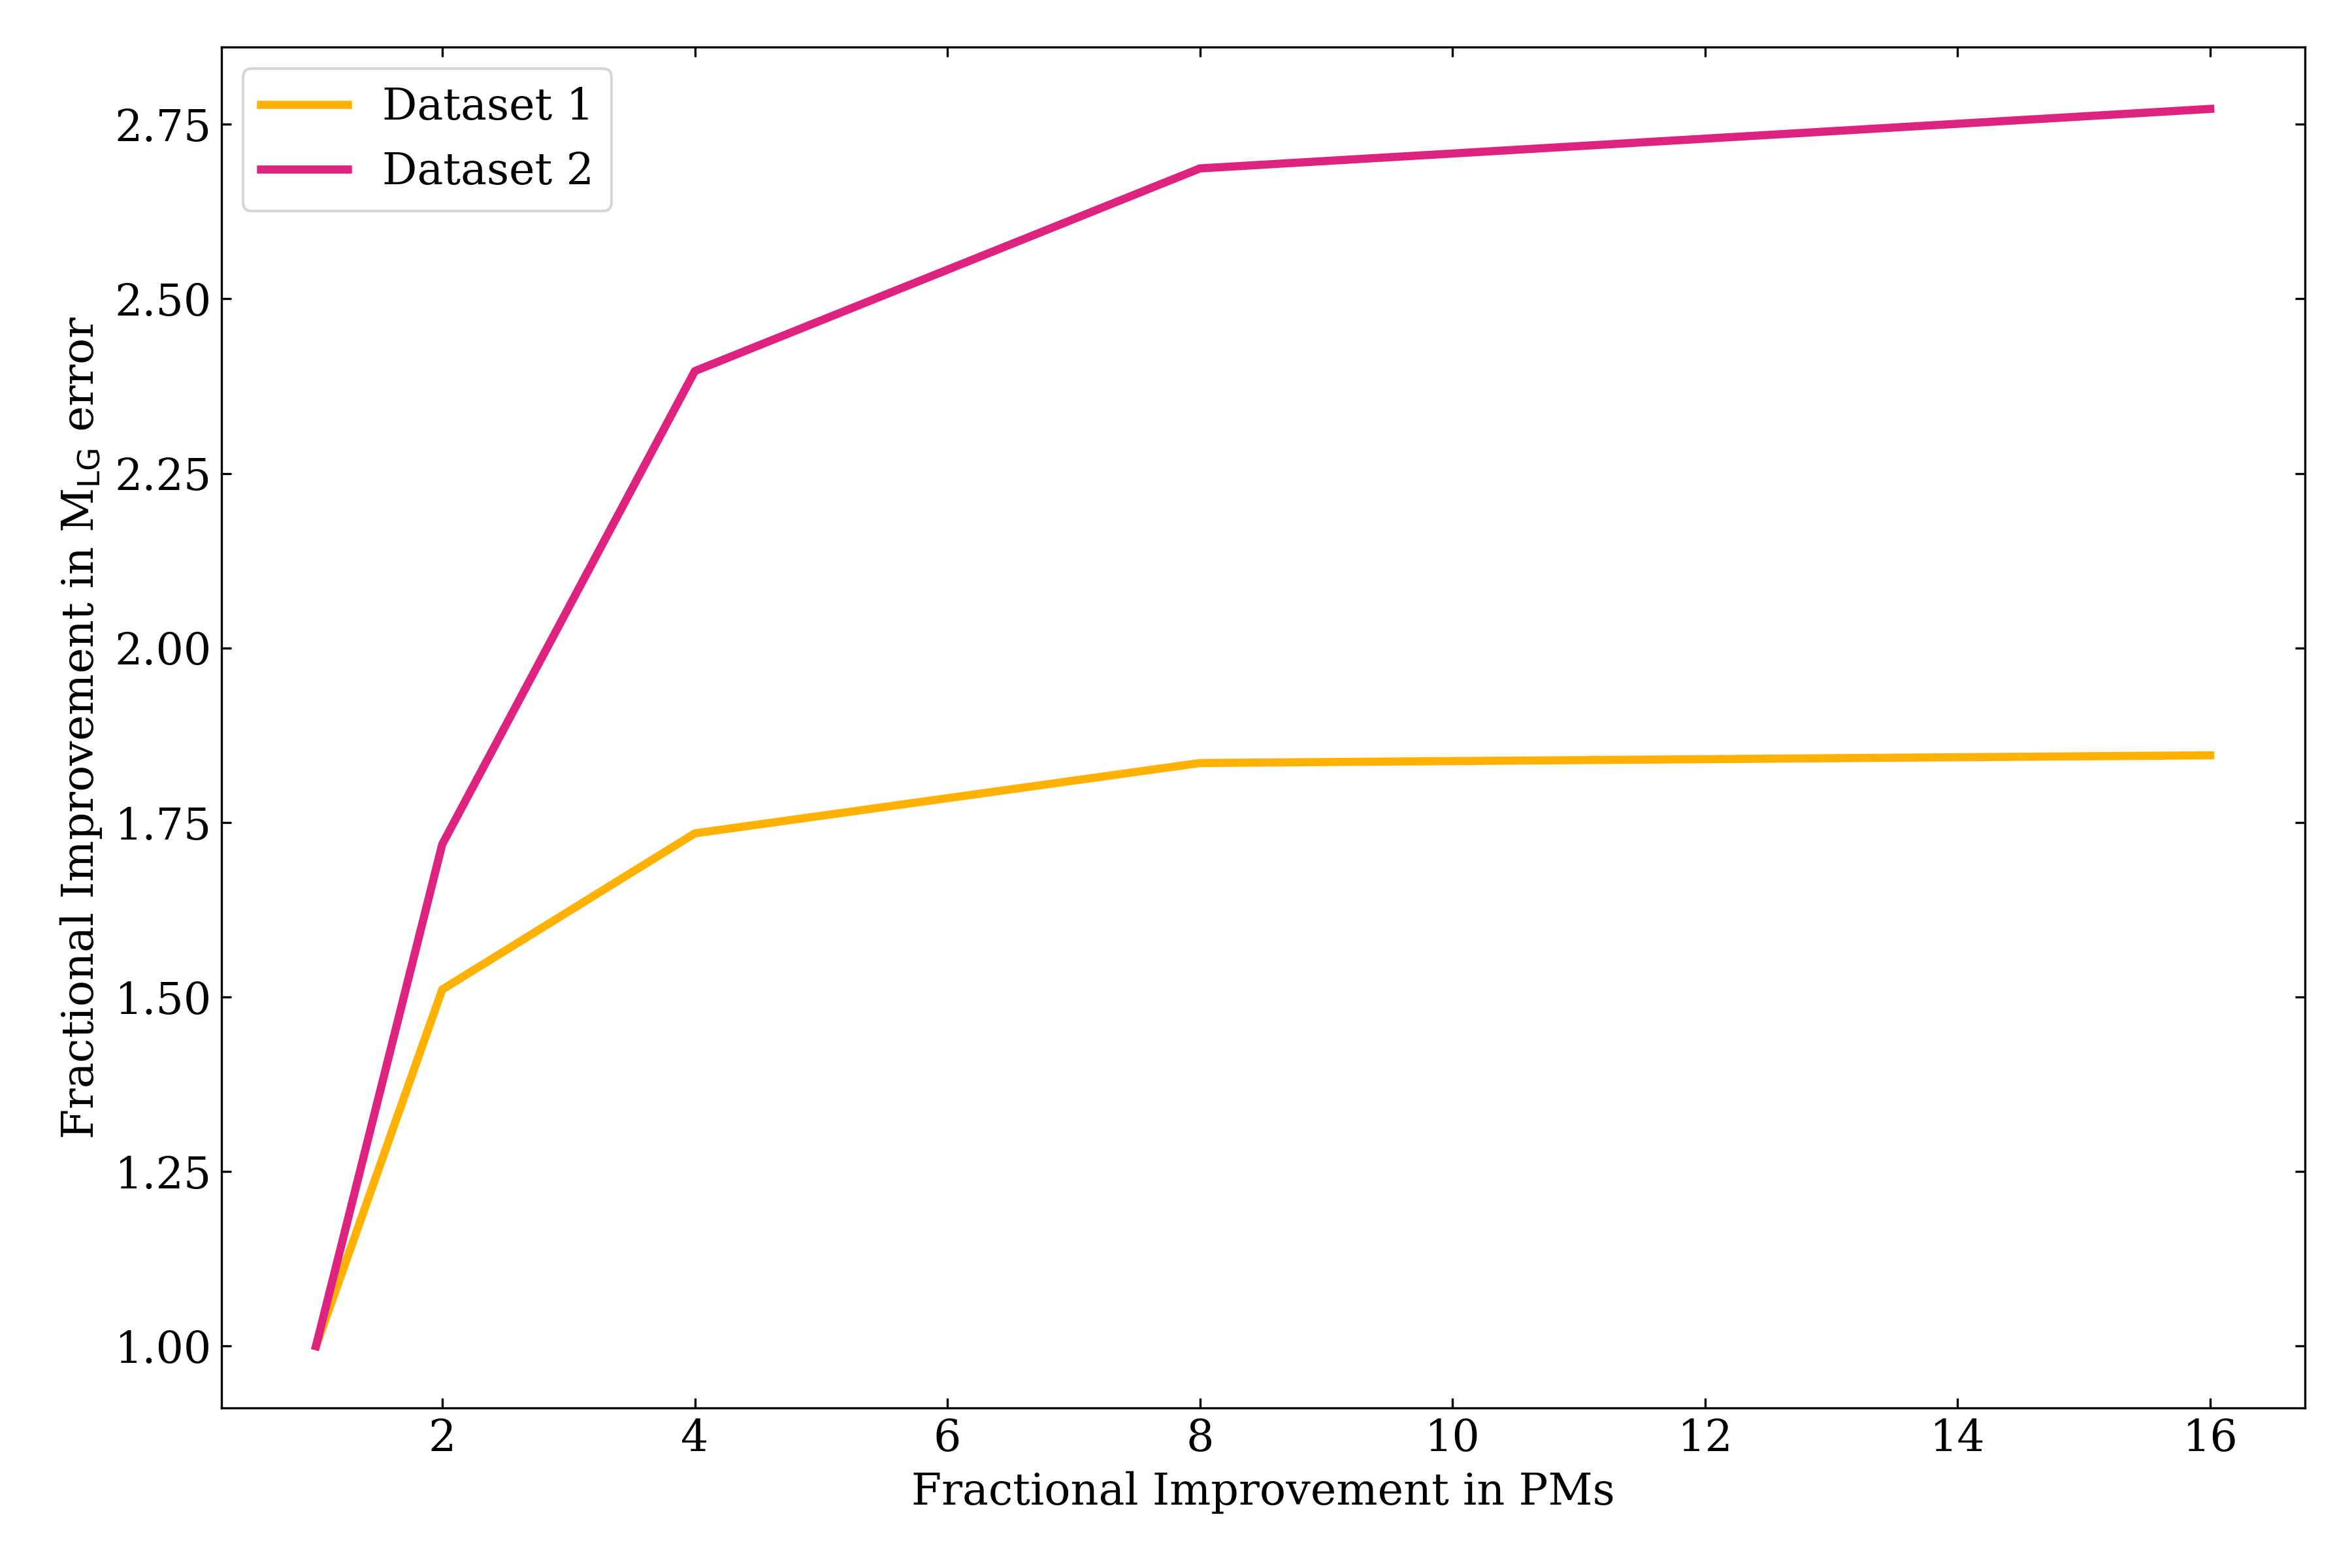
\includegraphics[width=\columnwidth]{analyze-runs-deltaMvsPM.png}
    \caption{\label{fig:mvspm} Improvement in the inferred Local Group mass as a function of fractional improvement in proper motion errors. The standard deviation in the mass decreases with decreasing proper motion error, and in particular, decrease by a factor of $\sim2.5$ for PMs that are 4 times smaller than in Dataset 2. \textbf{As future \textit{Gaia} data releases provide improved proper motion errors, constraints on the Local Group mass from the Timing Argument can improve by a factor of $>$2.}
    }
\end{figure}

%%%%%%%%%%%%%%%%%%%%%%%%%%%%%%%%%%%
\section{Summary and Discussion}
%%%%%%%%%%%%%%%%%%%%%%%%%%%%%%%%%%%
\label{sec:discussion}
In this Letter, we use the Timing Argument to constrain the mass of the Local 
Group by 
simplifying the dynamics of the MW--M31 pair to a Keplerian orbital model and 
given two compilations of data for the position and velocity of M31. 
However, these observations have not accounted for the reflex motion of the 
Milky Way disk with respect to the outer halo, and thus previous Timing
constraints on 
the LG mass do not include the crucial dynamical effect of the velocity boost 
of the disk.

We show that introducing the travel velocity of the MW disk into the Keplerian 
model lowers the inferred Local Group mass from the Timing Argument for two 6D
M31 datasets. 
We provide an updated constraint on the mass of the Local Group of 
4.69$\pm\times$0.71 $10^{12}\msun$ using recent \textit{Gaia} eDR3 proper 
motions~\citep{Salomon2021}, precise Cepheid distance measurements
~\citep{Li2021}, and assuming a disk travel velocity of 32km/s from
~\cite{Petersen2021}, and show that an increase in the travel velocity of the 
disk will result in even lower inferred LG masses.

\subsection{Cosmological implications}
\begin{table*}
  \centering
  \begin{tabular}{clc|c}
    \hline\hline
    Mass & Method & Result ($ 10^{12}\msun$ ) & Citation \\\hline
    \multirow{7}{*}{\mlg}  &{LV Galaxies + Timing Argument} & {2.64$\pm0.4$} & \cite{Penarrubia2016} \\
    &{Timing only} & {4.27$\pm$0.45} & \cite{vdm2012} \\
    &{Timing (3D + cosmic bias and scatter)} & {4.93$\pm$1.63} & \cite{vdm2012} \\
    &Timing (radial + cosmo sim calibration)  & $5.27$& \cite{LiWhite2008} \\
    &Timing & $3.6$ & \cite{Lynden-Bell:1981} \\
    & Cosmo Sims & 4.4$^{+2.4}_{-1.5}$ & \cite{Zhai2020}\\
    & LG Dynamics &$2.5\pm0.4$ & \cite{Diaz2014}\\
    %  &  &  \\
    \hline
    \multirow{3}{*}{\mmto}& Kinematics of M31 Sats & $1.4 \pm 0.4$ ($<$300 kpc) & \cite{Watkins2010}\\
    & Cosmo Sims & 2.5$^{+1.3}_{-1.1}$ & \cite{Zhai2020}\\
    & LG Dynamics &$1.7\pm0.3$ & \cite{Diaz2014}\\
    \hline
    \multirow{4}{*}{\mmw}&  Kinematics of LG sats & $1.4 \pm 0.3$ ($<$300 kpc) & \cite{Watkins2010}\\
    & Cosmo Sims & 1.5$^{+1.4}_{-0.7}$ & \cite{Zhai2020} \\
    & LG Dynamics &$0.8\pm0.5$ & \cite{Diaz2014}\\
    & MW Sats & $0.96^{+0.29}_{-0.28}$ & \cite{Patel2017}\\
  \hline\hline
  \end{tabular}
  \caption{\label{table:masses}Can remove this, this is just to keep me sane}
\end{table*}
Previous uses of the Timing Argument have placed constraints on the mass of the Local Group 

By including reflex motion, we move in the direction of the expected summed masses of the Milky Way and M31 which is good.

How does the mass that we found compare to mass estimates from other means? 
- like hubble flow constraints, previous timing argument, previous MW--M31 measurements, etc.



If our mass is higher, what does that mean? 
If our mass is lower, what does that mean?
What does this high mass mean to the Local Group? What about to the 
constituents? 

What is context for mergers and M31 and why they might be 
related to the Local Group mass?


Our findings of a high mass Local Group are consistent with findings that the 
mass of M31 is XXbig and the MW is $1-1.5\times10^{12}\msun$~\citep{??}. 
However, this high group mass also has cosmological implications. 
A high Local Group mass could also be consistent with tk that propose that M31 
has undergone recent (XX Gyrs) major? accretion events with other massive 
subhalos, resulting in morphological features like the Giant Southern Stream and 
XX (what are other M31 things that indicate recent interactions? Do we think 
much about M32? ) 

\subsection{Inclusion of reflex motion in dynamics of the Local Group}
The inclusion of the reflex motion of the Milky Way disk can result in up to 
$1\times10^{12}$ difference in the estimated mass of the Local Group, which 
means that by not accounting for this motion, we could get measurements of the 
Local group mass that are overestimated by 20-25\%.
Other dynamical interactions within the Local Group will also be affected by 
the reflex motion of the disk. (What is the distribution of satellite velocities 
about the MW now and w reflex motion? Cause should there maybe be an excess of 
-vrad satellites in the MW halo? )


\subsection{Expectations for future observations.}
\kc{Adrian!}

Do we expect Gaia DR3 proper motions to improve by a factor of ~4? 
This would provide the tightest constraints on the Local Group mass from the 
Timing Argument! 

\subsection{The M31--M33 system}
We do not account for the effects of reflex motion of M31 due to 
uncertainties in both its interaction history and the orbital history of 
M33. 
A first infall scenario for M33 would rule out the possibility of a 
strong reflex response resulting due to a close pericentric passage. 
On the other hand, M31 has likely experienced significant disturbances, as
evidenced by the double nucleus and Giant Southern Stream, 
which may have been resulted in a substantial reflex motion. 
Thus, we elect to disregard the effects of an M31 reflex motion. 


\subsection{Other?}
Concluding remarks



% \software{
%     Astropy \citep{astropy, astropy:2018},
%     gala \citep{gala},
%     IPython \citep{ipython},
%     numpy \citep{numpy},
%     pymc3 \citep{Salvatier2016},
%     scipy \citep{scipy}
% }

\bibliography{refs}{}
\bibliographystyle{aasjournal}

\end{document}
